\documentclass[12pt,a4paper,final,titlepage,twoside]{article}
\usepackage{MLABdoc}
\fancyhead[L]{{\huge LIGHTNING01A}}
\fancyfoot[RE,LO]{\today\hspace{1pt}|  | mlab.cz}

\includeonly{LIGHTNING01A.cs.title, LIGHTNING01A.cs.assembly}

\begin{document}
%vytvori uvodni stranku
\uvod
% nazev modulu
{LIGHTNING01A}
% kratky popis
{Detektor blesků}
%autor/i
{}
%obrazek
{../..//doc/img/LIGHTNING01A_QRcode.png}
%abstrakt
{Detektor blesků založený na integrovaném obvodu AS3935.}
%tabulka
{			io
		 & AS3935  & \\ \hline  }
%obrazek QR kodu
{../../doc/img/LIGHTNING01A_QRcode.png}


\section{Popis konstrukce}

\subsection{Zapojení}
Schéma zapojení je v příloze tohoto dokumentu.

\subsection{Mechanická konstrukce}

\section{Výroba a testování}

Tento modul umožňuje použití jak v režimu I2C, tak i v režimu SPI. Výběr režimu je proveden při výrobě modulu osazením určitých součástek.

\subsection{I2C}

\begin{center}
  \begin{tabular}{ | l | l | l | l |}
    \hline
    Označení & Hodnota, typ & Pouzdro & Počet \\ \hline
    \hline
			R1, R5 & 10k & SMD-0805 & 2\\ \hline
			R4 nebo R3 & 0 & SMD-0805 & 1\\ \hline
			R2 & R\_Small & SMD-0805 & 1\\ \hline
			R7, R8, R9 & 0 & SMD-0805 & 3\\ \hline
			R6 &  &  & 1\\ \hline
			D1 & M4 & Diode-MELF\_Standard & 1\\ \hline
			L1 & L\_Small & Coilcraft\_MA5532-AE\_RFID & 1\\ \hline
			J1 & JUMP2\_2x1 & Straight\_2x01 & 1\\ \hline
			J10 & JUMP\_3X2 & Straight\_2x03 & 1\\ \hline
			C4 & C/U & SMD-0805 & 1\\ \hline
			C1 & C\_Small & SMD-0805 & 1\\ \hline
			C5 & 100nF & SMD-0805 & 1\\ \hline
			C2 & 10uF & SMD-0805 & 1\\ \hline
			C3 & 1uF & SMD-0805 & 1\\ \hline
			U1 & AS3935 & MLPQ-16 & 1\\ \hline
			J2, J3 & - & Straight\_2x01 & 2\\ \hline
			J4, J5, J6, J7, J8, J9 & JUMP\_2x1 & Straight\_2x01 & 6\\ \hline
			M1, M2, M3, M4 & HOLE & MountingHole\_3mm & 4\\ \hline
	
  \end{tabular}
\end{center}
\subsection{SPI}

\begin{center}
  \begin{tabular}{ | l | l | l | l |}
    \hline
    Označení & Hodnota, typ & Pouzdro & Počet \\ \hline
    \hline
			R1, R4, R5, R6 & 0 & SMD-0805 & 1\\ \hline
			R2 & R\_Small & SMD-0805 & 1\\ \hline
			R3, R7, R8, R9 & - &  & 2\\ \hline
			D1 & M4 & Diode-MELF\_Standard & 1\\ \hline
			L1 & L\_Small & Coilcraft\_MA5532-AE\_RFID & 1\\ \hline
			J1 & - &  & 1\\ \hline
			J10 & JUMP\_3X2 & Straight\_2x03 & 1\\ \hline
			C4 & C/U & SMD-0805 & 1\\ \hline
			C1 & C\_Small & SMD-0805 & 1\\ \hline
			C5 & 100nF & SMD-0805 & 1\\ \hline
			C2 & 10uF & SMD-0805 & 1\\ \hline
			C3 & 1uF & SMD-0805 & 1\\ \hline
			U1 & AS3935 & MLPQ-16 & 1\\ \hline
			J2, J3, J4, J5, J6, J7, J8, J9 & JUMP\_2x1 & Straight\_2x01 & 8\\ \hline
			M1, M2, M3, M4 & HOLE & MountingHole\_3mm & 4\\ \hline	
  \end{tabular}
\end{center}

% totot naimportuje cast, kde jsou osazováky a BOM tabulka
\subsection{Osazení}


\begin{figure}[ht!]
	\centering
	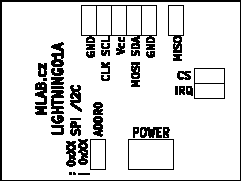
\includegraphics[scale=2]{../../doc/src/LIGHTNING01A-top_cropped.pdf}
	\qquad
	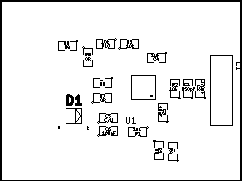
\includegraphics[scale=2]{../../doc/src/LIGHTNING01A-bottom_cropped.pdf}
\end{figure}

\begin{center}
  \begin{tabular}{ | l | l | l | l |}
    \hline
    Označení & Hodnota, typ & Pouzdro & Počet \\ \hline
    \hline
			R2, R1, R5, R10 & 10k & SMD-0805 & 4\\ \hline
			R7, R9, R8 & I2C & SMD-0805 & 3\\ \hline
			R4 & - & SMD-0805 & 1\\ \hline
			R6 & SPI & SMD-0805 & 1\\ \hline
			R3 & 0 & SMD-0805 & 1\\ \hline
			D1 & M4 & Diode-MELF\_Standard & 1\\ \hline
			L1 & 100uH & Coilcraft\_MA5532-AE\_RFID & 1\\ \hline
			J1 & JUMP2\_2x1 & Straight\_2x01 & 1\\ \hline
			J10 & JUMP\_3X2 & Straight\_2x03 & 1\\ \hline
			C5 & C/U & SMD-0805 & 1\\ \hline
			C2 & 270pF & SMD-0805 & 1\\ \hline
			C6 & 100nF & SMD-0805 & 1\\ \hline
			C1 & 650pF & SMD-0805 & 1\\ \hline
			C3 & 10uF & SMD-0805 & 1\\ \hline
			C4 & 1uF & SMD-0805 & 1\\ \hline
			U1 & AS3935 & MLPQ-16 & 1\\ \hline
			J2, J3, J4, J5, J6, J7, J8, J9 & JUMP\_2x1 & Straight\_2x01 & 8\\ \hline
			M1, M2, M3, M4 & HOLE & MountingHole\_3mm & 4\\ \hline
	
  \end{tabular}
\end{center}
\subsection{Nastavení}

\section{Programové vybavení}

%naimportuje schema 
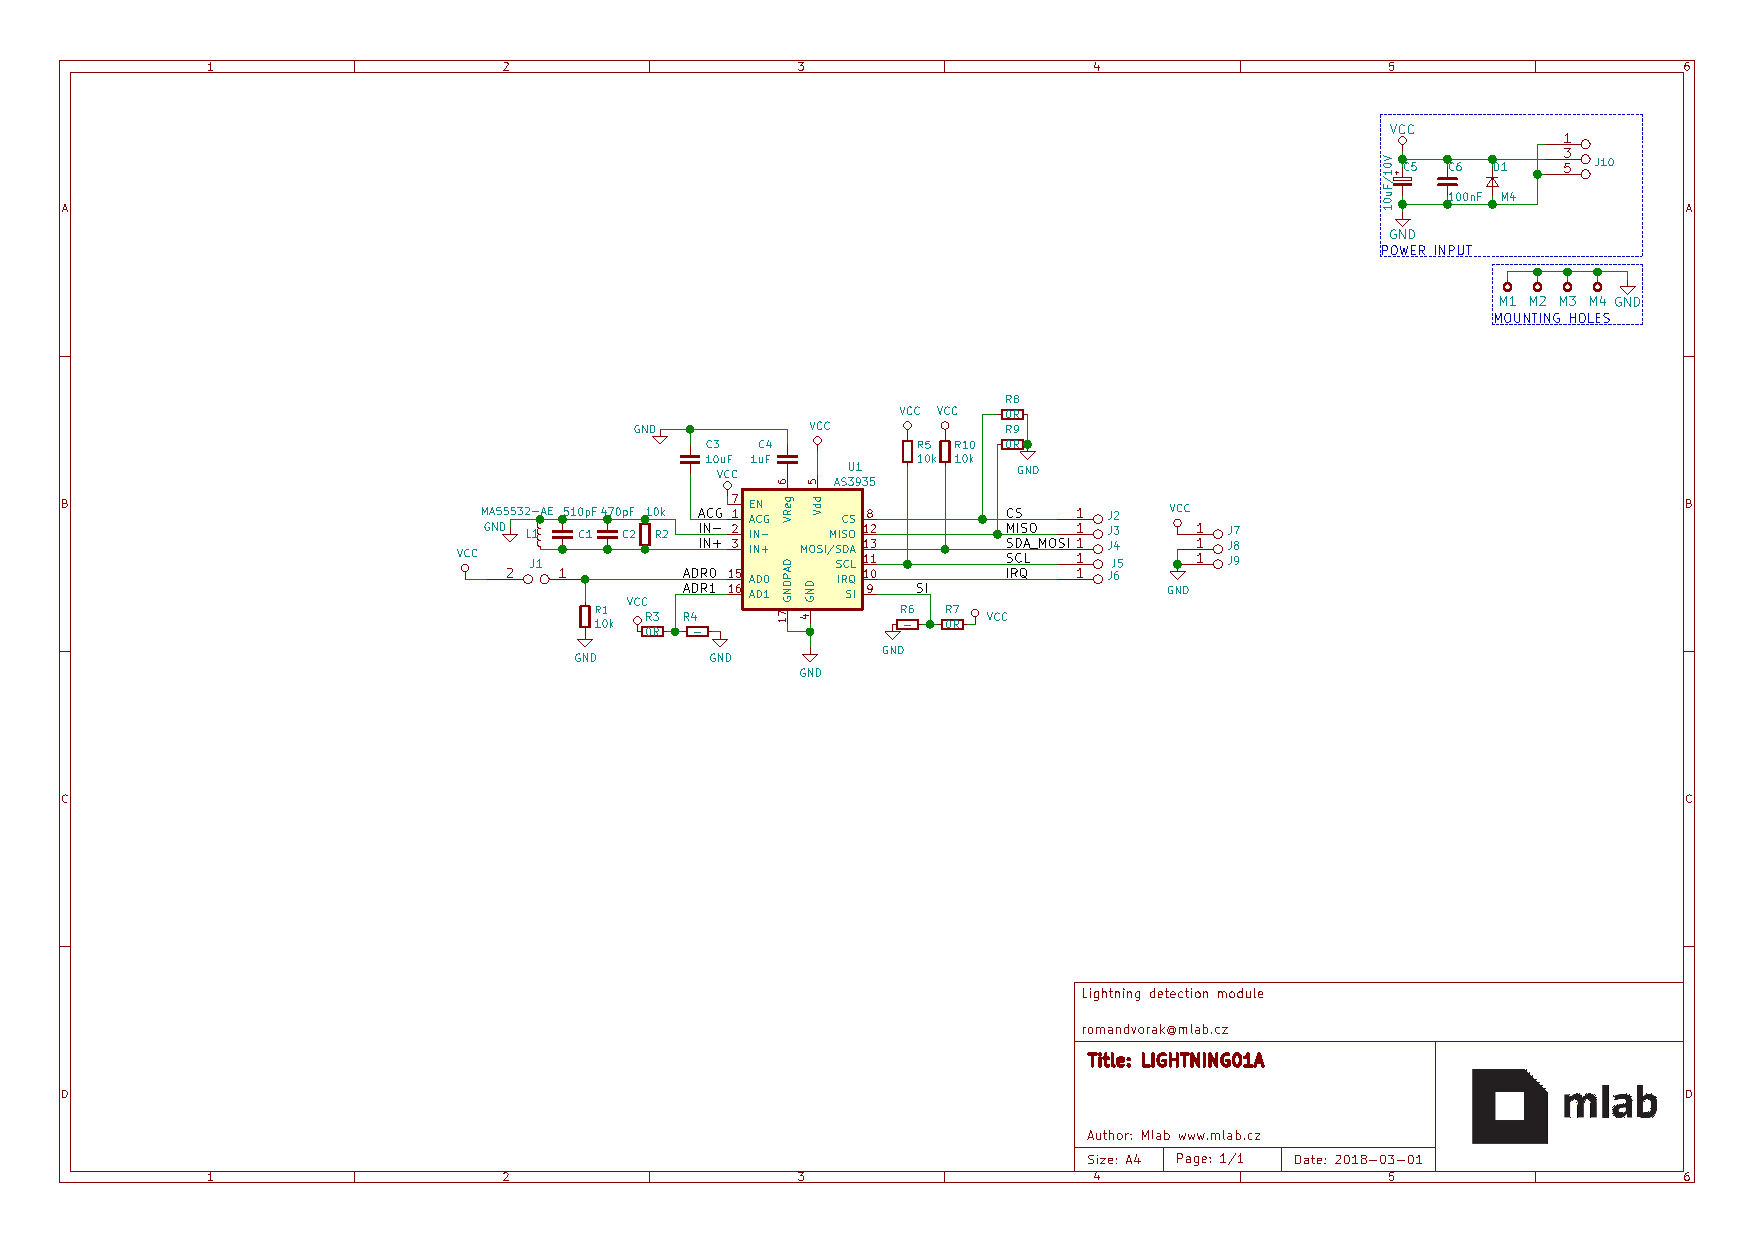
\includepdf[angle=90]{../../hw/sch_pcb/LIGHTNING01A.pdf}


\end{document}
